\section{INTRODUCTION}
\label{sec:INTRODUCTION}

%=======================
%--- Subsection 1.1 ---%
\subsection{Background of the Study}

Read \cref{sec:INTRODUCTION} for learning the basics of how to write in LaTeX and \cref{sec:REVIEW OF RELATED LITERATURE} for learning how to do citations. Moreover, glance \cref{sec:METHODOLOGY} and \cref{sec:RESULTS AND DISCUSSION} for manipulating figures and tables respectively.

Unless you know what you are doing, do not touch the Template folder, especially the preamble file as these files define the formatting. Replace the information for title page, abstract, keywords, and acknowledgment in main tex file with your own. Revise the Chapters, Tables, and Images folders as needed. Add your references data in the references.bib file.


%=======================
%--- Subsection 1.2 ---%
\subsection{Statement of the Problem}

\noindent Lists are easy to create:
\begin{itemize}
  \item List entries start with the \verb|\item| command.
  \item Individual entries are indicated with a black dot, a so-called bullet.
  \item The text in the entries may be of any length.
\end{itemize}


%=======================
%--- Subsection 1.3 ---%
\subsection{Objectives of the Study}

\noindent Numbered (ordered) lists are easy to create:
\begin{enumerate}
  \item Items are numbered automatically.
  \item The numbers start at 1 with each use of the \texttt{enumerate} environment.
  \item Another entry in the list
\end{enumerate}


%=======================
%--- Subsection 1.4 ---%
\subsection{Conceptual Framework}

    \begin{figure}[ht]
        \caption{Conceptual Framework of Camera-Based System With Voice Feedback}
        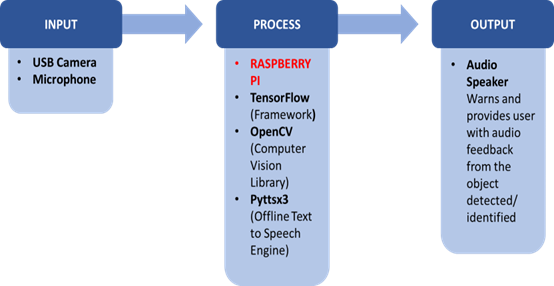
\includegraphics[width=1\textwidth]{Images/conceptual-framework.png}
        \label{fig:concept-frame}
    \end{figure}

You can put more than one value in the parameter, for instance, if you write [ht] LATEX will try to position the figure here, but if it's not possible (the space may be insufficient) then the figure will appear at the top of the page (See \autoref{table:pos-params} for more parameters). It is recommended to use more than one positioning parameter to prevent unexpected results.

To reference the figure, just call the label of the figure using \verb|\autoref|, i.e. \autoref{fig:concept-frame}, and it will automatically generate the correct reference. Resize the figure by changing this parameter \verb|[width=1\textwidth]| (this default means stretch the figure to occupy the whole width of the paper).


%=======================
%--- Subsection 1.5 ---%
\subsection{Significance of the Study}

    % insert the table for positioning parameters for Figures and Tables in LATEX
    \definecolor{ShuttleGray}{rgb}{0.364,0.407,0.474}
\begin{table}[ht]
\centering
\caption{Figure and Tables positioning parameters}
\begin{tblr}{
  width = \linewidth,
  colspec = {Q[69]Q[867]},
  cells = {fg=ShuttleGray},
  hline{2-8} = {-}{},
}
\textbf{Param} & \textbf{Position}                                                                                                                                                                                                                                                                                      \\
h              & \textcolor[rgb]{0.365,0.408,0.475}{Place the float~\textit{here\textcolor[rgb]{0.365,0.408,0.475}{, i.e.,~\textit{approximately\textcolor[rgb]{0.365,0.408,0.475}{~at the same point it occurs in the source text (however, not~\textit{exactly\textcolor[rgb]{0.365,0.408,0.475}{~at the spot)}}}}}}} \\
t              & \textcolor[rgb]{0.365,0.408,0.475}{Position at the~\textit{top\textcolor[rgb]{0.365,0.408,0.475}{~of the page.}}}                                                                                                                                                                                      \\
b              & \textcolor[rgb]{0.365,0.408,0.475}{Position at the~\textit{bottom\textcolor[rgb]{0.365,0.408,0.475}{~of the page.}}}                                                                                                                                                                                   \\
p              & \textcolor[rgb]{0.365,0.408,0.475}{Put on a special~\textit{page\textcolor[rgb]{0.365,0.408,0.475}{~for floats only.}}}                                                                                                                                                                                \\
!              & Override internal parameters LaTeX uses for determining "good" float positions.                                                                                                                                                                                                                        \\
H              & Places the float at precisely the location in the~LATEX~code. Requires the~float~package. This is somewhat equivalent to~h!.                                                                                                                                                                           
\end{tblr}
\label{table:pos-params}
\end{table}

Referencing tables is similar to referencing figures mentioned earlier, \autoref{table:pos-params}. To create hyperlinks, use \verb|\href| or \verb|\url|. For example, you can learn more about tables in this \href{https://www.overleaf.com/learn/latex/Tables}{link} or easily generate tables in LATEX format in this url: \url{https://www.latex-tables.com/}


%=======================
%--- Subsection 1.6 ---%
\subsection{Scope and Limitations}

Formulas should be used if they support the explanation. For formulas, LaTeX is ideal.
A formula should - if it is not extremely short - be presented in a separate line. For referencing, formulas should be numbered consecutively with Arabic numbers. The numbers should be aligned right in the last line of a formula. Formulas and variables must always be explained in the text.

Example: The following formula describes the expected mean snake length LQ of a (M/M/1) system, where represents the expected utilization:
\begin{equation}
       LQ=  \frac{\rho^2}{1-\rho} 
\end{equation}


%=======================
%--- Subsection 1.7 ---%
\subsection{Definition of Terms}

\noindent Change the labels using \verb|\item[label text]| in a \texttt{description} environment
\begin{description}
     \item[Note:] I would like to describe something here
     \item[Caveat!] And give a warning here
     \item[Term 1.] Lorem ipsum dolor sit amet, consectetur adipiscing elit, sed do eiusmod tempor incididunt ut labore et dolore magna aliqua.
     \item[Term 2.] Lorem ipsum dolor sit amet, consectetur adipiscing elit, sed do eiusmod tempor incididunt ut labore et dolore magna aliqua.
\end{description}